\chapter{Point by Point Method}

The point by point method will be applied to the HPS lamp. The candela table is presented in the Table~\ref{tab:hps_candela}.

\begin{table}
\centering
\begin{tabular}{|l|r|}
  \hline
  \textbf{Angle} & \textbf{Candela} \\
  \hline
  0 & 12984 \\
  \hline
  5 & 13072 \\
  \hline
  15 & 12892 \\
  \hline
  25 & 13402 \\
  \hline
  35 & 13033 \\
  \hline
  45 & 8792 \\
  \hline
  55 & 3584 \\
  \hline
  65 & 1355 \\
  \hline
  75 & 1379 \\
  \hline
  85 & 1572 \\
  \hline
  90 & 1638 \\
  \hline
  95 & 1686 \\
  \hline
  105 & 1721 \\
  \hline
  115 & 1682 \\
  \hline
  125 & 1560 \\
  \hline
  135 & 1416 \\
  \hline
  145 & 1361 \\
  \hline
  155 & 1042 \\
  \hline
  165 & 676 \\
  \hline
  175 & 339 \\
  \hline
  180 & 0 \\
  \hline
\end{tabular}
\caption{Candela table for the luminaire TH 400S PA22 (LEG 8, SC= 1.4).}
\label{tab:hps_candela}
\end{table}

\section{Lux Meter positioned under the luminaire}
Based on the candela Table~\ref{tab:hps_candela} and the Figure~\ref{fig:pp_under_lum}, the calculation of the illuminance for the groups of luminaires is presented by the Equations~\cref{eq:pp_under_point_a,eq:pp_under_point_b,eq:pp_under_point_c,eq:pp_under_point_d,eq:pp_under_point_e,eq:pp_under_point_f,eq:pp_under_lum}.

\begin{figure}[h!]
\centering
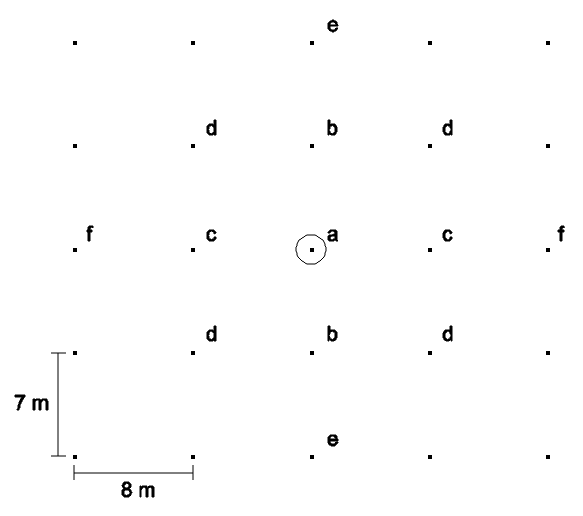
\includegraphics[width=.5\textwidth]{./figs/pp_under_lum.png}
\caption{Point by point method when the lux meter is under one luminaire.}
\label{fig:pp_under_lum}
\end{figure}

The Equation~\ref{eq:pp_under_point_a} presents the calculation for the point $a$.
\begin{equation}
\begin{split}
I_a &= \frac{I_{(cd)} \times \cos^3(\theta)}{H^2} \\
 &= \frac{12,984 \times \cos^3(0\degree)}{7.5^2} \\
 &= \frac{12,984}{56.25} \\
 & = 230.827 \\
 & \approx 230.83 lux
\end{split}
\label{eq:pp_under_point_a}
\end{equation}

The Equation~\ref{eq:pp_under_point_b} presents the calculation for the point $b$.
\begin{equation}
\begin{split}
\theta &= \tan^{-1}\left( \frac{Opposite}{Adjacent} \right) \\
 & = \tan^{-1}\left( \frac{7}{7.5} \right) \\
 & = 43.03\degree \\
 & \approx 43\degree\\
\\
x & = 43 \\
x_1 & = 35 \quad y_1 = 13,033 \\
x_2 & = 45 \quad y_2 = 8,792 \\
f(x) &= \frac{x_2 - x}{x_2 - x_1} \times y_1 +
       \frac{x - x_1}{x_2 - x_1} \times y_2 \\
 &= \frac{45 - 43}{45 - 35} \times 13,033 +
    \frac{43 - 35}{45 - 35} \times 8,792 \\
 & = 0.2 \times 13,033 - 0.8 \times 8,792 \\
 & = 9,632.2\: cd \\
\\
I_b &= \frac{I_{(cd)} \times \cos^3(\theta)}{H^2} \\
 &= \frac{9,632 \times \cos^3(43\degree)}{7.5^2} \\
 &= \frac{9,632 \times 0.39}{56.25} \\
 & = 66.986 \\
 & \approx 66.99\: lux
\end{split}
\label{eq:pp_under_point_b}
\end{equation}

The Equation~\ref{eq:pp_under_point_c} presents the calculation for the point $c$.
\begin{equation}
\begin{split}
\theta &= \tan^{-1}\left( \frac{Opposite}{Adjacent} \right) \\
 & = \tan^{-1}\left( \frac{8}{7.5} \right) \\
 & = 46.847\degree \\
 & \approx 47\degree\\
\\
x & = 47 \\
x_1 & = 45 \quad y_1 = 8,792 \\
x_2 & = 55 \quad y_2 = 3,584 \\
f(x) &= \frac{x_2 - x}{x_2 - x_1} \times y_1 +
       \frac{x - x_1}{x_2 - x_1} \times y_2 \\
 &= \frac{55 - 47}{55 - 45} \times 8,792 +
    \frac{47 - 45}{55 - 45} \times 3,584 \\
 & = 0.8 \times 8,792 - 0.2 \times 3,584 \\
 & = 7,750.4\: cd \\
\\
I_c &= \frac{I_{(cd)} \times \cos^3(\theta)}{H^2} \\
 &= \frac{7,750 \times \cos^3(47\degree)}{7.5^2} \\
 &= \frac{7,750 \times 0.31}{56.25} \\
 & = 43.707 \\
 & \approx 43.71\: lux
\end{split}
\label{eq:pp_under_point_c}
\end{equation}

The Equation~\ref{eq:pp_under_point_d} presents the calculation for the point $d$.
\begin{equation}
\begin{split}
s_{distance} & = \sqrt{8^2 + 7^2} \\
 & = \sqrt{113} \\
 & = 10.63 \\
\\
\theta &= \tan^{-1}\left( \frac{Opposite}{Adjacent} \right) \\
 & = \tan^{-1}\left( \frac{10.63}{7.5} \right) \\
 & = 54.795\degree \\
 & \approx 55\degree\\
\\
I_d &= \frac{I_{(cd)} \times \cos^3(\theta)}{H^2} \\
 &= \frac{3,584 \times \cos^3(55\degree)}{7.5^2} \\
 &= \frac{3,584 \times 0.19}{56.25} \\
 & = 12.023 \\
 & \approx 12.02\: lux
\end{split}
\label{eq:pp_under_point_d}
\end{equation}

The Equation~\ref{eq:pp_under_point_e} presents the calculation for the point $e$.
\begin{equation}
\begin{split}
s_{distance} = 14\\
\theta &= \tan^{-1}\left( \frac{Opposite}{Adjacent} \right) \\
 & = \tan^{-1}\left( \frac{14}{7.5} \right) \\
 & = 61.82\degree \\
 & \approx 62\degree\\
\\
x & = 62 \\
x_1 & = 55 \quad y_1 = 3,584 \\
x_2 & = 65 \quad y_2 =  1,355 \\
f(x) &= \frac{x_2 - x}{x_2 - x_1} \times y_1 +
       \frac{x - x_1}{x_2 - x_1} \times y_2 \\
 &= \frac{65 - 62}{65 - 55} \times 3,584 +
    \frac{62 - 55}{65 - 55} \times 1,355 \\
 & = 0.3 \times 3,584 - 0.7 \times 1,355 \\
 & = 2,023.7\: cd \\
\\
I_e &= \frac{I_{(cd)} \times \cos^3(\theta)}{H^2} \\
 &= \frac{2,023.7 \times \cos^3(62\degree)}{7.5^2} \\
 &= \frac{2,023.7 \times 0.104}{56.25} \\
 & = 3.723 \\
 & \approx 3.72\: lux
\end{split}
\label{eq:pp_under_point_e}
\end{equation}

The Equation~\ref{eq:pp_under_point_f} presents the calculation for the point $f$.
\begin{equation}
\begin{split}
s_{distance} = 16\\
\theta &= \tan^{-1}\left( \frac{Opposite}{Adjacent} \right) \\
 & = \tan^{-1}\left( \frac{16}{7.5} \right) \\
 & = 64.885\degree \\
 & \approx 65\degree\\
\\
I_f &= \frac{I_{(cd)} \times \cos^3(\theta)}{H^2} \\
 &= \frac{1,355 \times \cos^3(65\degree)}{7.5^2} \\
 &= \frac{1,355 \times 0.075}{56.25} \\
 & = 1.818 \\
 & \approx 1.82\: lux
\end{split}
\label{eq:pp_under_point_f}
\end{equation}

The Equation~\ref{eq:pp_under_lum} presents the calculation for the total illumination contribution.
\begin{equation}
\begin{split}
I_{total} &= I_a + 2 \times I_b + 2 \times I_c + 4 \times I_d + 2 \times I_e + 2 \times I_f \\
 &= 230.83 + 2 \times 66.99 + 2 \times 43.71 + 4 \times 12.02 + 2 \times 3.72 + 2 \times 1.82 \\
 & = 511.39 \\
\end{split}
\label{eq:pp_under_lum}
\end{equation}

\section{Lux Meter positioned between two luminaires}
Based on the candela Table~\ref{tab:hps_candela} and the Figure~\ref{fig:pp_between_2_lum}, the calculation of the illuminance for the groups of luminaires is presented by the Equations~\cref{eq:pp_between_2_point_a,eq:pp_between_2_point_b,eq:pp_between_2_point_c,eq:pp_between_2_point_d,eq:pp_between_2_point_e,eq:pp_between_2_point_f,eq:pp_between_2_lum}.

\begin{figure}[h!]
\centering
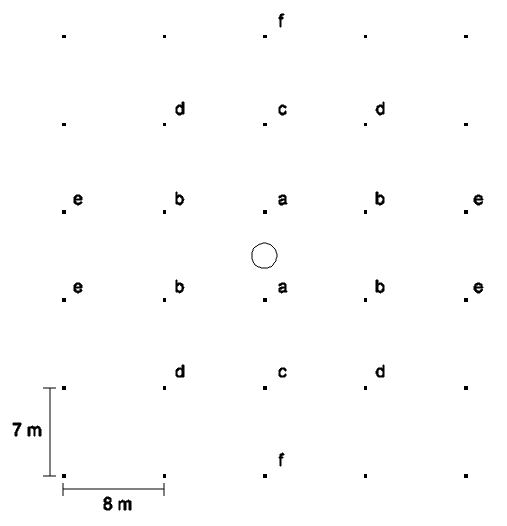
\includegraphics[width=.5\textwidth]{./figs/pp_between_2_lum.png}
\caption{Point by point method when the lux meter is between two luminaires.}
\label{fig:pp_between_2_lum}
\end{figure}

The Equation~\ref{eq:pp_between_2_point_a} presents the calculation for the point $a$.
\begin{equation}
\begin{split}
s_{distance} = 3.5\\
\theta &= \tan^{-1}\left( \frac{Opposite}{Adjacent} \right) \\
 & = \tan^{-1}\left( \frac{3.5}{7.5} \right) \\
 & = 25.16\degree \\
 & \approx 25\degree\\
\\
I_a &= \frac{I_{(cd)} \times \cos^3(\theta)}{H^2} \\
 &= \frac{13,402 \times \cos^3(25\degree)}{7.5^2} \\
 &= \frac{13,402 \times 0.74}{56.25} \\
 & = 177.368 \\
 & \approx 177.37 lux
\end{split}
\label{eq:pp_between_2_point_a}
\end{equation}

The Equation~\ref{eq:pp_between_2_point_b} presents the calculation for the point $b$.
\begin{equation}
\begin{split}
s_{distance} & = \sqrt{3.5^2 + 8^2} \\
 & = \sqrt{76.25} \\
 & = 8.73 \\
\\
\theta &= \tan^{-1}\left( \frac{Opposite}{Adjacent} \right) \\
 & = \tan^{-1}\left( \frac{8.73}{7.5} \right) \\
 & = 49.334\degree \\
 & \approx 49\degree\\
\\
x & = 49 \\
x_1 & = 45 \quad y_1 = 8,792 \\
x_2 & = 55 \quad y_2 = 3,584 \\
f(x) &= \frac{x_2 - x}{x_2 - x_1} \times y_1 +
       \frac{x - x_1}{x_2 - x_1} \times y_2 \\
 &= \frac{55 - 49}{55 - 45} \times 8,792 +
    \frac{49 - 45}{55 - 45} \times 3,584 \\
 & = 0.6 \times 8,792 - 0.4 \times 3,584 \\
 & = 6,708.8\: cd \\
\\
I_b &= \frac{I_{(cd)} \times \cos^3(\theta)}{H^2} \\
 &= \frac{6,708.8 \times \cos^3(49\degree)}{7.5^2} \\
 &= \frac{6,708.8 \times 0.28}{56.25} \\
 & = 33.678 \\
 & \approx 33.68\: lux
\end{split}
\label{eq:pp_between_2_point_b}
\end{equation}

The Equation~\ref{eq:pp_between_2_point_c} presents the calculation for the point $c$.
\begin{equation}
\begin{split}
s_{distance} = 10.5\\
\theta &= \tan^{-1}\left( \frac{Opposite}{Adjacent} \right) \\
 & = \tan^{-1}\left( \frac{10.5}{7.5} \right) \\
 & = 54.46\degree \\
 & \approx 55\degree\\
\\
I_c &= \frac{I_{(cd)} \times \cos^3(\theta)}{H^2} \\
 &= \frac{3,584 \times \cos^3(55\degree)}{7.5^2} \\
 &= \frac{3,584 \times 0.19}{56.25} \\
 & = 12.023 \\
 & \approx 12.023\: lux
\end{split}
\label{eq:pp_between_2_point_c}
\end{equation}

The Equation~\ref{eq:pp_between_2_point_d} presents the calculation for the point $d$.
\begin{equation}
\begin{split}
s_{distance} & = \sqrt{10.5^2 + 8^2} \\
 & = \sqrt{174.25} \\
 & = 13.2 \\
\\
\theta &= \tan^{-1}\left( \frac{Opposite}{Adjacent} \right) \\
 & = \tan^{-1}\left( \frac{12.2}{7.5} \right) \\
 & = 60.396\degree \\
 & \approx 60\degree\\
\\
x & = 60 \\
x_1 & = 55 \quad y_1 = 3,584 \\
x_2 & = 65 \quad y_2 = 1,355 \\
f(x) &= \frac{x_2 - x}{x_2 - x_1} \times y_1 +
       \frac{x - x_1}{x_2 - x_1} \times y_2 \\
 &= \frac{65 - 60}{65 - 55} \times 3,584 +
    \frac{60 - 55}{65 - 55} \times 1,355 \\
 & = 0.5 \times 3,584 - 0.5 \times 1,355 \\
 & = 2,469.5\: cd \\
\\
I_d &= \frac{I_{(cd)} \times \cos^3(\theta)}{H^2} \\
 &= \frac{2,469.5 \times \cos^3(60\degree)}{7.5^2} \\
 &= \frac{2,469.5 \times 0.125}{56.25} \\
 & = 5.488 \\
 & \approx 5.49\: lux
\end{split}
\label{eq:pp_between_2_point_d}
\end{equation}

The Equation~\ref{eq:pp_between_2_point_e} presents the calculation for the point $e$.
\begin{equation}
\begin{split}
s_{distance} & = \sqrt{3.5^2 + 16^2} \\
 & = \sqrt{268.25} \\
 & = 16.38 \\
\theta &= \tan^{-1}\left( \frac{Opposite}{Adjacent} \right) \\
 & = \tan^{-1}\left( \frac{16.38}{7.5} \right) \\
 & = 65.398\degree \\
 & \approx 65\degree\\
\\
I_e &= \frac{I_{(cd)} \times \cos^3(\theta)}{H^2} \\
 &= \frac{1,355 \times \cos^3(65\degree)}{7.5^2} \\
 &= \frac{1,355 \times 0.075}{56.25} \\
 & = 1.818 \\
 & \approx 1.82\: lux
\end{split}
\label{eq:pp_between_2_point_e}
\end{equation}

The Equation~\ref{eq:pp_between_2_point_f} presents the calculation for the point $f$.
\begin{equation}
\begin{split}
s_{distance} = 17.5\\
\theta &= \tan^{-1}\left( \frac{Opposite}{Adjacent} \right) \\
 & = \tan^{-1}\left( \frac{17.5}{7.5} \right) \\
 & = 66.801\degree \\
 & \approx 67\degree\\
\\
x & = 67 \\
x_1 & = 65 \quad y_1 = 1,355 \\
x_2 & = 75 \quad y_2 = 1,379 \\
f(x) &= \frac{x_2 - x}{x_2 - x_1} \times y_1 +
       \frac{x - x_1}{x_2 - x_1} \times y_2 \\
 &= \frac{75 - 67}{75 - 65} \times 1,355 +
    \frac{67 - 65}{75 - 65} \times 1,379 \\
 & = 0.8 \times 1,355 - 0.2 \times 1,379 \\
 & = 1,359.8\: cd \\
\\
I_f &= \frac{I_{(cd)} \times \cos^3(\theta)}{H^2} \\
 &= \frac{1,359.8 \times \cos^3(67\degree)}{7.5^2} \\
 &= \frac{1,359.8 \times 0.06}{56.25} \\
 & = 1.442 \\
 & \approx 1.44\: lux
\end{split}
\label{eq:pp_between_2_point_f}
\end{equation}

The Equation~\ref{eq:pp_between_2_lum} presents the calculation for the total illumination contribution.
\begin{equation}
\begin{split}
I_{total} &= 2 \times I_a + 4 \times I_b + 2 \times I_c + 4 \times I_d + 4 \times I_e + 2 \times I_f \\
 &= 2 \times 177.37 + 4 \times 33.68 + 2 \times 12.02 + 4 \times 5.49 + 4 \times 1.82 + 2 \times 1.44 \\
 & = 545.62 \\
\end{split}
\label{eq:pp_between_2_lum}
\end{equation}

\section{Lux Meter positioned between four luminaires}
Based on the candela Table~\ref{tab:hps_candela} and the Figure~\ref{fig:pp_between_4_lum}, the calculation of the illuminance for the groups of luminaires is presented by the Equations~\cref{eq:pp_between_4_point_a,eq:pp_between_4_point_b,eq:pp_between_4_point_c,eq:pp_between_4_point_d,eq:pp_between_4_point_e,eq:pp_between_4_lum}.

\begin{figure}[h!]
\centering
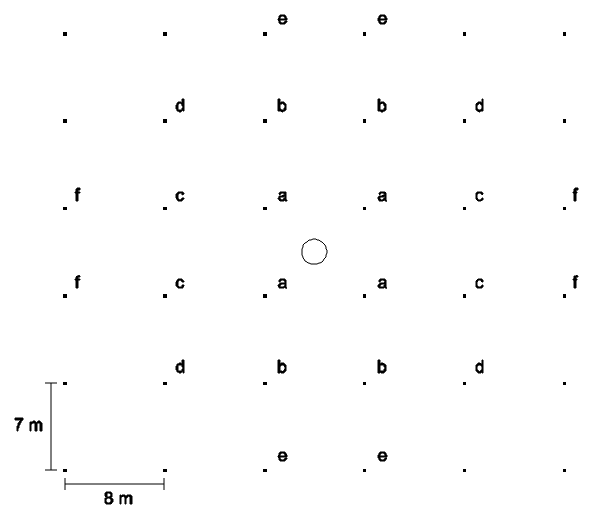
\includegraphics[width=.5\textwidth]{./figs/pp_between_4_lum.png}
\caption{Point by point method when the lux meter is between four luminaires.}
\label{fig:pp_between_4_lum}
\end{figure}

The Equation~\ref{eq:pp_between_4_point_a} presents the calculation for the point $a$.
\begin{equation}
\begin{split}
s_{distance} & = \sqrt{3.5^2 + 4^2} \\
 & = \sqrt{28.25} \\
 & = 5.32 \\
\theta &= \tan^{-1}\left( \frac{Opposite}{Adjacent} \right) \\
 & = \tan^{-1}\left( \frac{5.32}{7.5} \right) \\
 & = 35.349\degree \\
 & \approx 35\degree\\
\\
I_a &= \frac{I_{(cd)} \times \cos^3(\theta)}{H^2} \\
 &= \frac{13,033 \times \cos^3(35\degree)}{7.5^2} \\
 &= \frac{13,033 \times 0.55}{56.25} \\
 & = 127.355 \\
 & \approx 127.36 lux
\end{split}
\label{eq:pp_between_4_point_a}
\end{equation}

The Equation~\ref{eq:pp_between_4_point_b} presents the calculation for the point $b$.
\begin{equation}
\begin{split}
s_{distance} & = \sqrt{3.5^2 + 10.5^2} \\
 & = \sqrt{122.25} \\
 & = 11.07 \\
\\
\theta &= \tan^{-1}\left( \frac{Opposite}{Adjacent} \right) \\
 & = \tan^{-1}\left( \frac{10.07}{7.5} \right) \\
 & = 55.88\degree \\
 & \approx 56\degree\\
\\
x & = 56 \\
x_1 & = 55 \quad y_1 = 3,584 \\
x_2 & = 65 \quad y_2 = 1,355 \\
f(x) &= \frac{x_2 - x}{x_2 - x_1} \times y_1 +
       \frac{x - x_1}{x_2 - x_1} \times y_2 \\
 &= \frac{65 - 56}{65 - 55} \times 3,584 +
    \frac{56 - 55}{65 - 55} \times 1,355 \\
 & = 0.9 \times 3,584 - 0.1 \times 1,355 \\
 & = 3,361.1\: cd \\
\\
I_b &= \frac{I_{(cd)} \times \cos^3(\theta)}{H^2} \\
 &= \frac{3,361.1 \times \cos^3(56\degree)}{7.5^2} \\
 &= \frac{3,361.1 \times 0.17}{56.25} \\
 & = 10.448 \\
 & \approx 10.45\: lux
\end{split}
\label{eq:pp_between_4_point_b}
\end{equation}

The Equation~\ref{eq:pp_between_4_point_c} presents the calculation for the point $c$.
\begin{equation}
\begin{split}
s_{distance} & = \sqrt{3.5^2 + 12^2} \\
 & = \sqrt{156.25} \\
 & = 12.5 \\
\\
\theta &= \tan^{-1}\left( \frac{Opposite}{Adjacent} \right) \\
 & = \tan^{-1}\left( \frac{12.5}{7.5} \right) \\
 & = 59.04\degree \\
 & \approx 59\degree\\
\\
x & = 59 \\
x_1 & = 55 \quad y_1 = 3,584 \\
x_2 & = 65 \quad y_2 = 1,355 \\
f(x) &= \frac{x_2 - x}{x_2 - x_1} \times y_1 +
       \frac{x - x_1}{x_2 - x_1} \times y_2 \\
 &= \frac{65 - 59}{65 - 55} \times 3,584 +
    \frac{59 - 55}{65 - 55} \times 1,355 \\
 & = 0.6 \times 3,584 - 0.4 \times 1,355 \\
 & = 2,692.4\: cd \\
\\
I_c &= \frac{I_{(cd)} \times \cos^3(\theta)}{H^2} \\
 &= \frac{2,692.4 \times \cos^3(59\degree)}{7.5^2} \\
 &= \frac{2,692.4 \times 0.14}{56.25} \\
 & = 6.539 \\
 & \approx 6.54\: lux
\end{split}
\label{eq:pp_between_4_point_c}
\end{equation}

The Equation~\ref{eq:pp_between_4_point_d} presents the calculation for the point $d$.
\begin{equation}
\begin{split}
s_{distance} & = \sqrt{10.5^2 + 12^2} \\
 & = \sqrt{254.25} \\
 & = 15.95 \\
\\
\theta &= \tan^{-1}\left( \frac{Opposite}{Adjacent} \right) \\
 & = \tan^{-1}\left( \frac{15.95}{7.5} \right) \\
 & = 64.816\degree \\
 & \approx 65\degree\\
\\
I_d &= \frac{I_{(cd)} \times \cos^3(\theta)}{H^2} \\
 &= \frac{1,355 \times \cos^3(65\degree)}{7.5^2} \\
 &= \frac{1,355 \times 0.075}{56.25} \\
 & = 1.818 \\
 & \approx 1.82\: lux
\end{split}
\label{eq:pp_between_4_point_d}
\end{equation}

The Equation~\ref{eq:pp_between_4_point_e} presents the calculation for the point $e$.
\begin{equation}
\begin{split}
s_{distance} & = \sqrt{3.5^2 + 17.5^2} \\
 & = \sqrt{318.25} \\
 & = 17.85 \\
\theta &= \tan^{-1}\left( \frac{Opposite}{Adjacent} \right) \\
 & = \tan^{-1}\left( \frac{17.85}{7.5} \right) \\
 & = 67.209\degree \\
 & \approx 67\degree\\
\\
x & = 67 \\
x_1 & = 65 \quad y_1 = 1,355 \\
x_2 & = 75 \quad y_2 = 1,379 \\
f(x) &= \frac{x_2 - x}{x_2 - x_1} \times y_1 +
       \frac{x - x_1}{x_2 - x_1} \times y_2 \\
 &= \frac{75 - 67}{75 - 65} \times 1,355 +
    \frac{67 - 65}{75 - 65} \times 1,379 \\
 & = 0.8 \times 1,355 - 0.2 \times 1,379 \\
 & = 1,359.8\: cd \\
\\
I_e &= \frac{I_{(cd)} \times \cos^3(\theta)}{H^2} \\
 &= \frac{1,359.8 \times \cos^3(67\degree)}{7.5^2} \\
 &= \frac{1,359.8 \times 0.06}{56.25} \\
 & = 1.442 \\
 & \approx 1.44\: lux
\end{split}
\label{eq:pp_between_4_point_e}
\end{equation}

The Equation~\ref{eq:pp_between_4_lum} presents the calculation for the total illumination contribution.
\begin{equation}
\begin{split}
I_{total} &= 4 \times I_a + 4 \times I_b + 4 \times I_c + 4 \times I_d + 4 \times I_e \\
 &= 4 \times 127.36 + 4 \times 10.45 + 4 \times 6.54 + 4 \times 1.82 + 4 \times 1.44 \\
 & = 590.44 \\
\end{split}
\label{eq:pp_between_4_lum}
\end{equation}

\section{Uniformity Test}
The Equation~\ref{eq:test_unif} presents the uniformity test calculation.
\begin{equation}
\begin{split}
T &= \frac{I_{bigger\,value} - I_{lower\,value}}{I_{lower\,value}} \\
 &= \frac{590.44 - 511.39}{511.39} \\
 & = 0.1546 \\
 & \approx 15.46\%
\end{split}
\label{eq:test_unif}
\end{equation}
The result of the Equation~\ref{eq:test_unif} shows that this project has uniformity, because the test is lower than $30\%$.



